\documentclass{article}
\usepackage[nonatbib]{nips_2016}

\usepackage[breaklinks=true,letterpaper=true,colorlinks,citecolor=black,bookmarks=false]{hyperref}

\usepackage{amsthm}
\usepackage{amsmath,amssymb}
\usepackage{enumitem}

\usepackage[sort&compress,numbers]{natbib}
\usepackage[normalem]{ulem}

% use Times
\usepackage{times}
% For figures
\usepackage{graphicx} % more modern
%\usepackage{epsfig} % less modern
%\usepackage{subfig}

\graphicspath{{../fig/}}

\usepackage{tikz}
\usepackage{tkz-tab}
\usepackage{caption}
\usepackage{subcaption}
\usetikzlibrary{shapes.geometric, arrows}
\tikzstyle{arrow} = [very thick,->,>=stealth]

\usepackage{cleveref}
\usepackage{setspace}
\usepackage{wrapfig}
%\usepackage[ruled]{algorithm}
\usepackage{algpseudocode}
\usepackage[noend,linesnumbered]{algorithm2e}

\usepackage[disable]{todonotes}

\usepackage{algpseudocode}

\usepackage{amsmath}
\usepackage{booktabs}
\usepackage{multirow}
\usepackage{titlesec}

\newcommand{\red}[1]{\textcolor{red}{#1}}



\title{Dynamic Model Construction for Efficient Classification}

\author{
    Jaejun Lee \\
    School of Computer Science\\
    University of Waterloo\\
    Waterloo, ON, N2L 3G1 \\
    \texttt{j474lee@uwaterloo.ca} \\
}

\begin{document}
\maketitle

\begin{abstract}

One of the major drawback of neural network in the domain of classification is that retraining is unavoidable when the target set of class changes. For this reason, networks are often designed to be wide and deep. However, this leads to increase the necessary computations which has a direct impact on the efficiency of the model. In this work, I study how different combination of loss function and last activation function affects the classification output and present a new way to add or remove a class from target class set without retraining. With this technique, a model can be adjusted to classify any combination of target classes and the minimal resource usage is guaranteed as the adjusted model involves the same amount of computations as the model trained to classify the same set of class explicitly.

\end{abstract}

\section{Introduction}

Current issues


In this section you are going to present a brief background and motivation of your project. Why is it interesting/significant? How does it relate to the course?

\section{Related Works}

The main challenge with this problem is on model flexibility and resource usage. Even though these two aspects are quite related, they are generally considered as two separate problem. As a result, this problem can be categorized differently depending on which direction one approaches. The three most related domains are: ensemble learning, multi-task learning, and transfer learning

\subsection{Ensemble Learning}
Ensemble learning is a common technique in the field of machine learning which achieves greater performance by combining outputs from multiple models which are independent. The most famous techniques are voting, weighting, bagging and boosting~\cite{dietterich2000ensemble, breiman1996bagging, freund1996experiments}. Even though ensemble learning is considered to be easy to implement, most of the ensemble techniques assume that each model has different architecture. As a result, ensemble learning often requires significant computations as it requires every model to process the input.

\subsection{Multi-task Learning}
On the other hand, multi-task learning takes different approach; combining multiple models into a single model. The key assumption is that if tasks are related, sharing information among tasks throughout training will increase the performance on each task. There are numbers of variations depending on the assumptions. Key design choices include: what kind of information to share and how much information to share among tasks. Two main categories of multi-task learnings are parameter sharing and feature sharing~\cite{ruder2017overview, Caruana1993MultitaskLA, duong2015low, lu2017fully} which differ by type of the information that are shared. Even though multi-task learning has the similar architecture with the desired solution, it is hard to adopt it as a solution for our problem, due to it's assumption that the each task are distinct.

\subsection{Transfer Learning}

Transfer learning is inspired by the same assumption as in multi-task learning; if tasks are related, sharing knowledge improves the performance. However, the key difference between two problem is that transfer learning are designed to share the same model architecture for different tasks. First, a model is pre-trained with a task and learns to select important features. Then the model is fine-tuned for the target task, putting all of its effort to produce the best result for the target task exploiting selected features~\cite{yosinski2014transferable}. With its architectural flexibility, transfer learning has been adopted in wide domains and has shown its strengths~\cite{raina2007self, egan2004effects, glorot2011domain}.

\section{Dynamic Model Construction with Class-level Transfer Learning}

\subsection{Approach}

In this section, I introduce how to achieve dynamic model construction which adopts to the change in target class set.

One of the common technique used for multi-task learning is to use distinct fully-connected layer for each task~\cite{huang2016mtnet, girshick2015fast, long2017learning}. In this setting, each task is trained independently while weights for upstream layers are shared among classes. Once model is trained, a task can be discarded from populating output if it is no longer necessary. This is achieved simply by removing corresponding fully-connected layer.

Next consider a case of transfer learning. Pre-training a model and fine-tuning for target task can leads to increase in performance. There is no change in model architecture throughout this process. Therefore, fine-tuned model uses the same amount of computation as the model which is explicitly trained to accomplish the same task.

Exploiting these characteristics in two distinct domains, the proposed algorithm can be summarized as following:

\begin{enumerate}
    \item pre-train a model as if it is targeting multi-classification problem
    \item freeze the model parameters
    \item fine-tune a model to obtain class-specific weights (step 4 $\sim$ 7)
    \item construct a dataset which labels corresponding class as positive and the others as negative.
    \item replace the last full-connected layer with two classes
    \item fine-tune the last layer with the constructed data
    \item store weights for positive class
    \item at the time of the inference, the last fully-connected layer is dynamically constructed to classify the given set of class by loading corresponding weights obtained from fine-tuning
\end{enumerate}

For simplicity, I will call this algorithm as composing algorithm, the model trained for multi-class as base model, models constructed from step 4 $\sim$ 7 as fine-tuned models and the model constructed from the last step as composed model.

\red{to be raised in introduction}

Recall that the desired composed model should satisfy the following conditions:

\begin{enumerate}
    \item \red{preserve accuracy}
    \item Dynamic addition and removal of a class must be possible
    \item Minimal computation is desired for an inference
\end{enumerate}

Addition and removal of a class is possible with the composing algorithm as it can be achieved simply by adding or removing corresponding fully-connected connections.
With such a simply addition, retraining the base model is no longer necessary, which is unavoidable in the previous setting. Furthermore, note that even though a class does not contributes to step 1, it can be fine-tuned and added for step 8 as long as the same base model is used for fine-tuning.

From fine-tuning and composing, we only work with the last full-connected layer; when a model is fine-tuned for a class, the weights we store are from the fully-connected layer.
Since we do not use weights trained for negative class, the architecture of the composed model is same as the base model, assuming that the composed model is designed to classify all classes which base model is trained for. Therefore, we can conclude that the composed model does not add any computations compared to the base model.

\section{Accuracy Preservation}

The most challenging part with the composable model problem is assuring that the composed model suffers from the minimal change in accuracy. In this section, I discuss how such condition can be satisfied with the algorithm presented in the previous section.

\subsection{Limitations with cross entropy loss}

State of the art loss for multi-classification problem is cross entropy (CE) loss, which transforms output using softmax and calculates loss using negative log likelihood (NLL).
Softmax and NLL loss are defined as following:

\begin{align*}
Softmax(y_i) &= \frac{e^{y_i}}{\sum_{j}e^{y_j}} \\
NegativeLogLikelihood(y, t) & = -\frac{1}{N}\sum_{i=1}^N \left[ t_i \cdot \log y_i\right] \\
\end{align*}

where $x$ is the output of the network and $t$ is the target. target is one hot encoded vector as in common classification problem.

Softmax is normalized logits computed from the output of the network. Therefore each index has value between zero and one and sum is designed to be one. Since multi-class classifier rely on the mutually exclusive assumption with about the classes, CE loss is the most suitable as it promotes the positive class while suppressing the negative classes.

However, such assumption does not hold for composed model and CE loss can cause indeterministic behaviour with composed model. When CE loss is used throughout the composing algorithm, the loss which used in fine-tuning is computed with respect to the output of negative class. However, for a composed model, it is not fair to select the class with the greatest value as final class because model outputs for each class are not constructed with respect to each other.

For example, let us say there are 3 classes: A, B, and C. For fine-tuning, we construct a dataset which has two classes: one for target class (positive class) and the other constructed with the other two classes (negative class). Once models are fine-tuned for each class, we have weights for positive class and negative class. For simplicity, positive weights are referred with lower case (a, b, and c) and negative weights with lower case with prime (a', b', and c'). During fine-tuning, loss is calculated in pairs: a -- a', b -- b', c -- c'. However, when we construct a composed model, the last layer consists of weights a, b and c. As a results, selecting the highest value as a final class is not a valid approach.

\subsection{Binary cross entropy with sigmoid}

We now understand the limitation of CE loss caused by mutually exclusive assumption among classes. To overcome such issue, I propose binary cross entropy (BCE) loss with sigmoid.

\begin{align*}
Sigmoid(y_i) &= \frac{1}{1 + e^{-x_i}} \\
BinaryCrossEntropy(y, t) & = -\frac{1}{N}\sum_{i=1}^N \left[ t_i \cdot \log y_i + (1 - t_i) \cdot \log (1 - t_i) \right] \\
\end{align*}

Unlike softmax in CE Loss, the only input for sigmoid is the output from the network at the corresponding index. Furthermore, while CE loss considers mutually exclusive assumption as part of its calculation, BCE loss considers each index independently and is calculated with respect to its target. As a result, weights for each class in fine-tuned model no longer depend on other factors. This indicates that class with the highest output from composed model has the highest probability of being true class.

It is found that multi-label classification has raised the same issue with CE loss~\cite{liu2017deep}. It is found that the independence guarantee provided by BCE loss with sigmoid is crucial for multi-label classification and enabled successful training of a model.

\section{Experiments}

Realising the theoritical limitation of cross entropy loss, I have conducted thorough experiments using PyTorch, reporting how different loss function affects the performance of composed model.

In this experiment, I evaluate three different loss functions. First loss function is CE loss. Since PyTorch NLL loss implementation expects log probability, log is applied after softmax but it is found that this does not affect the conclusion from the experiments. Next, I include sigmoid with BCE loss which successfully preserves accuracy between base and composed model. Lastly, I include BCE loss with softmax. This setting is known to be unstable because BCE loss assumes the independence among classes. In fact, I have observed the training collapse once it reaches a certain point. However, since we report accuracy from the best model, results from this setting is still valid and meaningful. This setting should demonstrate how crucial sigmoid is in the composing algorithm as it simply replace sigmoid with softmax from last setting.

Experiments are conducted with MNIST, Keyword Spotting, and CIFAR100 varying on number of classes, 10, 30, and, 100 respectively. From each experiment, I report accuracy of base model, fine-tuned model, and composed model. Furthermore, as I construct composed model by adding a class at a time, I also report accuracy for each intermediary composed model to understand how how number of classes affects the accuracy of combined model. It is found that the intermediary composed model accuracy fluctuate quite a bit depending on the order each class is added. Therefore, I repeat this process 10 times for each base model as I randomly select a class to add next.


% To reduce the effects of outliers, experiments are conducted multiple times and average results are included in this report. Due to the limited time, number of iterations are different for each experiment and discussed along with other data specific experimental setting in the following section.

\subsection{MNIST}

MNIST is a standard benchmark for classification~\cite{lecun1998gradient} which consist of images for handwritten digits. Among the wide range of model architecture solving this problem, I have conducted my experiments with LeNet-5 ~\cite{lecun2015lenet}. LeNet-5 is constructed with two convolutional, one dropout and two fully connected layers. The original implementation of LeNet-5 has 10 and 20 channels for the two convolutional layers and produces accuracy of 98\% on MNIST dataset. Since our goal of this experiment is to understand the difference in peformance caused by different loss functions, I intentionally limited the expressive power of the network by constructing the network with only 5 channels for both convolutional layers.

Both base model training and fine-tuning is conducted using Adam optimizer with learning rate of 0.0001. It is found that 5 epochs are enough for each training to be converged and LeNet-5 achieves average accuracy of 95\% with the base model and 98\% with the fine-tuned model (see Figure \ref{table:mnist_base} and \ref{table:mnist_fine_tuned}). In fact, all three loss functions present similar accuracy confirming that the comparison on the composed model is fair.

Figure \ref{table:mnist_base} summarizes how the accuracy changes as number of classes increases for composed model. No matter which loss function is used for composing algorithm, decrease in accuracy is found as more classes are involved for the composed model construction. However, models with softmax based loss is found to suffer at a greater rate than models with sigmoid based loss. With CE loss, the composed model for all 10 classes has an accuracy of 85.86\% introducing about 10\% decrease compared to the base model. BCE loss with softmax is found to be the least effective for composing algorithm as it leads to final accuracy of 78.50\%. On the other hand, BCE loss with sigmoid introduces the minimal degradation and achieves the finall accuracy of 95.29\%. This proves that class independence training is crucial with the composing algorithm.

\begin{table}[t]
    \mbox{}\hfill
    \begin{minipage}[c]{0.49\textwidth}
        \centering{\ttfamily
            \begin{tabular}{cc}
                \toprule[1pt]
                \bf{Loss function} &
                \bf{Base model} \\
                \midrule
                LogSoftmax + NLL & 95.82 \\
                Softmax + BCE & 94.86 \\
                Sigmoid + BCE & 95.48 \\
                \bottomrule[1pt]
            \end{tabular}
    }
    \end{minipage}
    \hfill
    \begin{minipage}[c]{0.49\textwidth}
        \centering
        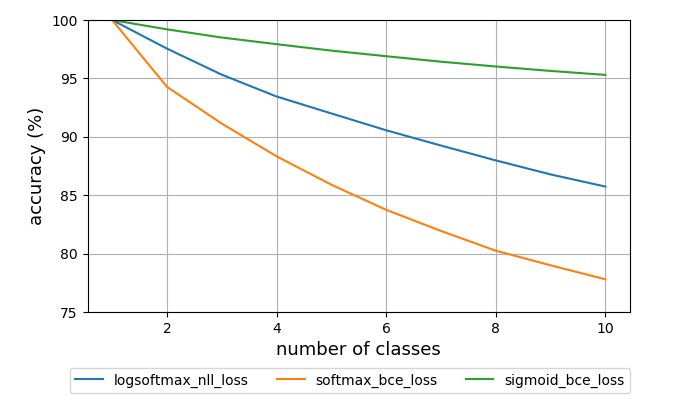
\includegraphics[scale=0.4,trim={0mm 0mm 0mm 0mm},clip]{mnist.png}
    \end{minipage}
    \hfill
    \mbox{}

    \caption{Accuracy of base model(left) and composed model with respect to number of classes(right)}
    \label{table:mnist_base}
\end{table}

\begin{table*}[t]
    \centering
    \small
    \scalebox{0.9}{
        \begin{tabular}{ccccccccccc}
            \toprule[1pt]
            \multirow{2}{*}{\raisebox{-3\heavyrulewidth}{\bf Loss function}} &
            \multicolumn{10}{c}{\bf Fine tuned model } \\
            \cmidrule(lr){2-11}
            & 0 & 1 & 2 & 3 & 4 & 5 & 6 & 7 & 8 & 9 \\
            \midrule
            LogSoftmax + NLL & 99.04 & 99.23 & 97.79 & 98.18 & 98.09 & 98.03 & 98.64 & 97.74 & 97.12 & 96.34 \\
            Softmax + BCE & 98.81 & 99.09 & 97.23 & 97.60 & 97.45 & 97.04 & 98.34 & 97.32 & 96.46 & 95.44 \\
            Sigmoid + BCE & 99.03 & 99.19 & 97.68 & 98.21 & 98.31 & 98.09 & 98.54 & 97.57 & 97.18 & 96.66 \\
            \bottomrule[1pt]
        \end{tabular}
    }
    \caption{Accuracy of fine-tuned model per each class}
    \label{table:mnist_fine_tuned}
\end{table*}



\subsection{Keyword Spotting}

\subsubsection{Experimental Setup}

\subsubsection{Experimental results}


\begin{table}[t]
    \mbox{}\hfill
    \begin{minipage}[c]{0.49\textwidth}
        \centering{\ttfamily
            \begin{tabular}{cc}
                \toprule[1pt]
                \bf{Loss function} &
                \bf{Base model} \\
                \midrule
                LogSoftmax + NLL & 94.03 \\
                Softmax + BCE & 91.84 \\
                Sigmoid + BCE & 90.82 \\
                \bottomrule[1pt]
            \end{tabular}
    }
    \end{minipage}
    \hfill
    \begin{minipage}[c]{0.49\textwidth}
        \centering
        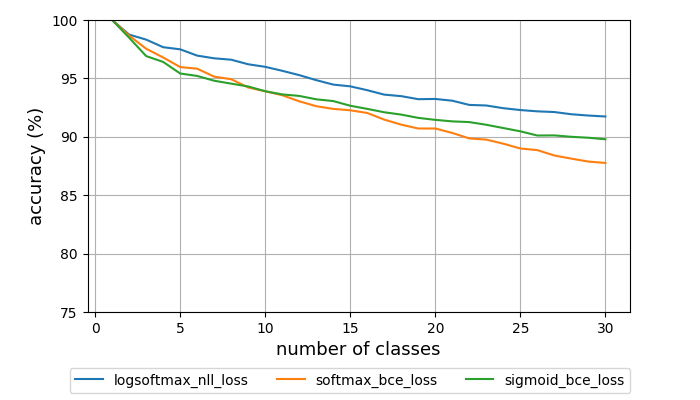
\includegraphics[scale=0.4,trim={0mm 0mm 0mm 0mm},clip]{res15.png}
    \end{minipage}
    \hfill
    \mbox{}

    \caption{Accuracy of base model(left) and composed model with respect to number of classes(right)}
    \label{table:kws_base}
\end{table}

\subsection{CIFAR100}

densenet ~\cite{huang2017densely}
\subsubsection{Experimental Setup}

\subsubsection{Experimental results}



\section{Conclusion}
In this section please concisely describe what you are going to achieve in this project. E.g., formulate your problem precisely (mathematically), present the technical challenges (if any), discuss the tools or datasets that you will build on, state your goals, and come up with a plan for evaluation.

For your own sake, you might want to lay out a time line, so that you can keep a good track of your project.

\newpage

\section*{Acknowledgement}
Thank people who have helped or influenced you in this project.

\nocite{*}

\bibliographystyle{unsrtnat}
\bibliography{citation}

\end{document}
